\documentclass[twoside]{report}
\usepackage[italian]{babel}
\usepackage[utf8]{inputenc}
\usepackage{amsmath}
\usepackage{amsthm}
\usepackage{amsfonts}
\usepackage{amssymb}
\usepackage{cancel}
\usepackage[margin=1in]{geometry}
\usepackage{hyperref}
\usepackage{bookmark}
\usepackage{setspace}
\usepackage{titlesec}
\usepackage{hyperref}
\usepackage{graphicx}
\usepackage{fancyhdr}
\usepackage{float}


\graphicspath{{./images/}}

\setlength{\parskip}{0pt}
\titlespacing*{\subparagraph}{1.25em}{0em}{0.35em} 

\makeatletter
\renewenvironment{abstract}{%
    \if@twocolumn
        \section*{\abstractname}%
    \else
        \begin{center}%
            {\bfseries \abstractname\vspace{-.5em}\vspace{\z@}}%
        \end{center}%
        \small
        \begin{quotation}
    \fi}
    {\if@twocolumn\else\end{quotation}\fi}
\makeatother

\fancypagestyle{chapterInit}{%
    \fancyhf{}
    \renewcommand{\headrulewidth}{0pt}
    \fancyfoot{}
    \fancyfoot[LE,RO]{\thepage}
    \fancyfoot[LO,RE]{"Appunti di Introduction to Computer and Network Security" di Luca Facchini}
    \renewcommand{\footrulewidth}{0.4pt}
}
\fancypagestyle{stdPageS}{
    \fancyhead{}
    \fancyhead[RO,LE]{\leftmark}
    \fancyfoot{}
    \fancyfoot[LE,RO]{\thepage}
    \fancyfoot[LO,RE]{"Appunti di Introduction to Computer and Network Security" di Luca Facchini}
    \renewcommand{\footrulewidth}{0.4pt}
}

\addtocontents{toc}{\protect\thispagestyle{stdPageS}}

\title{Appunti di Introduction to Computer and Network Security}
\author{Luca Facchini (mat. 245965)}
\date{A.A. 2024/2025}

\hypersetup{
    pdfauthor={Luca Facchini},
    pdftitle={Appunti di Introduction to Computer and Network Security},
    pdfsubject={Appunti del corso di Introduction to Computer and Network Security tenuto dal prof. Raniese Silvio presso l'Università degli Studi di Trento nell'anno accademico 2024/2025.},
    pdfkeywords={Computer Security, Network Security, Introduction to Computer and Network Security, UniTN, Università degli Studi di Trento},
    pdfproducer={LaTeX},
    pdfcreator={pdflatex},
}

\begin{document}
    \begin{titlepage}
        \centering  % Center everything on the title page
        {\Huge\textbf{Appunti di Introduction to Computer and Network Security}} \\[1cm] % Title
        \vspace{0.5cm}
        
        {\Large Luca Facchini} \\ % Author name
        \vspace{0.3cm}
        {\large Matricola: 245965} \\[2cm] % Additional author info
        
        {\large Corso tenuto dal prof. Raniese Silvio} \\[0.3cm] % Course information
        {\large Università degli Studi di Trento} \\[1.5cm]
        
        {\large A.A. 2024/2025} \\[3cm] % Academic year
        
        % Abstract section with spacing control
        \vfill
        \begin{abstract}
            Appunti del corso di Introduction to Computer and Network Security tenuto dal prof. Raniese Silvio presso l'Università degli Studi di Trento nell'anno accademico 2024/2025.
        \end{abstract}
        
        \vfill  % Pushes the content to the center vertically
    \end{titlepage}
    \pagestyle{stdPageS}
    \begingroup
        \setcounter{tocdepth}{1}
        \tableofcontents
    \endgroup
    \chapter{Basic Notions - Nozioni Base}
\thispagestyle{chapterInit}
\section{The CIA Triad}
\label{sec:ciaTriad}
    \subsection{Introduzione}
    \paragraph{L'acronimo} L'acronimo CIA in inglese sta per \textbf{Confidentiality}, \textbf{Integrity} e \textbf{Availability}. Questi tre concetti sono alla base della sicurezza informatica e della protezione dei dati.  
        \subparagraph{Confidentiality - Riservatezza}
        \label{subPar:confidentiality}
            Il principio della Riservatezza prescrive che i non autorizzati non devono poter accedere ai dati e i dati sono visibili solo a chi è autorizzato a vederli.
        \subparagraph{Integrity - Integrità}
        \label{subPar:integrity}
            Il principio di Integrità prescrive che i dati non devono essere modificati se non da persone autorizzate a farlo, i tentativi di modifica non autorizzati devono essere rilevati e prevenuti.
        \subparagraph{Availability - Disponibilità}
            Il principio della Disponibilità prescrive che i dati non devono essere mantenuti inaccessibili ed inoltre bisogna permettere l'accesso agli autorizzati alle informazioni e ai servizi.
    \subsection{In Pratica}
        \paragraph{Confidentiality - Riservatezza}
            L'accesso alle informazioni riservare può essere:
            \subparagraph{Intenzionale} Quando un intruso cerca di accedere a dati sensibili.
            \subparagraph{Non Intenzionale} Quando un utente autorizzato accede a dati sensibili senza volerlo causato dal fatto che chi detiene i dati non è competente e/o non gli importa della sicurezza.
        
            Come garantire la riservatezza:
            \subparagraph{Crittografia} La \textbf{crittografia} è una tecnica che permette di limitare l'accesso ai dati solo a chi possiede la chiave per decifrarli (e quindi è autorizzato).
            \subparagraph{Access Control} Il \textbf{controllo degli accessi} è una parte integrante per mantenere la \textbf{riservatezza}, ciò andando a gestire quali utenti possono accedere a quali risorse.
        \paragraph{Integrity - Integrità}
            Per garantire l'integrità bisogna prevenire la modifica e/o la distruzione, inoltre bisogna assicurare informazioni autentiche e non invalidate.

            Inoltre ulteriore prescrizione è quella di individuare anche le cosiddette "minute changes" ovvero le modifiche minime che possono essere fatte ai dati per alterarne il significato. 
            
            L'integrità può essere anche di tipo \textbf{data integrity} ovvero la garanzia che i dati siano corretti e completi, oppure di tipo \textbf{system integrity} ovvero la garanzia che il sistema sia protetto da attacchi e che funzioni correttamente.

            L'itemize può essere compromessa da:
            \begin{itemize}
                \item errore umano
                \item attacchi come malware distruttivi e ransomware
            \end{itemize}
            Come garantire l'integrità:
            \subparagraph{Version Control} Il \textbf{controllo delle versioni} assieme agli \textbf{audit trails} permettono ad una organizzazione di garantire la veridicità dei dati.
            \subparagraph{Compliance requirements} I \textbf{requisiti di conformità} sono regole e normative che un'organizzazione deve seguire per garantire l'integrità dei dati.
        \paragraph{Availability - Disponibilità}
            Le violazioni alla disponibilità includono:
            \begin{itemize}
                \item Fallimento dell'infrastruttura 
                \item Overload dell'infrastruttura
                \item Blackout
                \item Attacchi come DDoS
            \end{itemize}
            Come garantire la disponibilità:
            \subparagraph{Backup} Bisogna sempre avere un piano di \textbf{backup} per mantenere disponibile in caso di disastro, attacco o altre minacce si verificassero.
            \subparagraph{Cloud} Il \textbf{cloud} è una soluzione per garantire la disponibilità dei dati, in quanto i dati sono replicati su più server e quindi in caso di guasto di uno di essi i dati sono comunque disponibili.
        
\section{Security Policy, Mechanism, Service}
    \subsection{Security Policy}
            \subsubsection{Definizione}
                Una \textbf{security policy} è un insieme di regole e requisiti stabilita da una azienda che definisce l'uso accettabile delle informazioni e dei servizi, inoltre il livello indica il livello di confidenzialità, integrità e disponibilità delle informazioni.
            \subsubsection{Esempi}
                Un esempio di possibili regole di una \textbf{security policy} potrebbero essere:
                \begin{itemize}
                    \item I dipendenti devono completare il corso su sicurezza informatica e accettare la policy di sicurezza.
                    \item I visitatori dell'azienda devono essere accompagnati da un dipendente autorizzato in tutti i momenti, questo dipendente deve mantenere i visitatori in una area appropriata senza dati sensibili
                    \item I dipendenti devono mantenere una "scrivania pulita" dunque senza lasciare documenti sensibili accessibili e incustoditi.
                    \item I dipendenti devono usare una password sicura e queste non devono essere usate in altri servizi esterni.
                    \item Gli ex-dipendenti non devono mantenere alcun dato dell'azienda.
                \end{itemize}
    \subsection{Security Service}
            \subsubsection{Definizione} La capacità di supportare uno o più dei requisiti di sicurezza (Confidentiality, Integrity, Availability) e.s.: gestione chiavi, controllo accessi, autenticazione.
                Come già detto i \textbf{Security Services} implementano uno o più \textbf{Security Mechanism} che servono per far rispettare la \textbf{Security Policy}.
            \subsubsection{Esempi}
                \paragraph{HTTP(S)}
                    \subparagraph{HTTP} Se si sua il protocolla \textbf{HTTP} per la trasmissione dei dati qualsiasi informazione trasmessa può venire intercettata da hacker nel mezzo.
                    \subparagraph{HTTPS} Per ovviare a questo problema si usa il protocollo \textbf{HTTPS} che è una versione sicura di \textbf{HTTP} che usa la crittografia per proteggere i dati, in questo modo i dati trasmessi vengono cifrati e se intercettati non possono essere letti.
                \paragraph{Access Control}
                    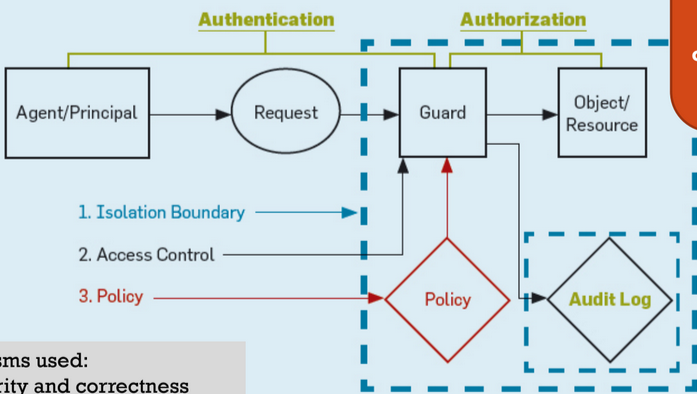
\includegraphics[height=12.5em]{01/accessControlSchema.png}
                    \subparagraph{Audit Log} è un registro importante che registra tutte le richieste di accesso ai dati e se la richiesta è stata accettata o rifiutata, in questo modo si può monitorare se una richiesta che è stata fatta ha avuto un risultato non aspettato e quindi che vadano modificate le \textbf{policy}.
    \subsection{Security Mechanism}
    \label{subsec:securityMechanism}
        \subsubsection{Definizione} Un \textbf{security mechanism} un dispositivo o funzione designato per provvedere uno o più servizi di sicurezza classificate in termini di potenza
            
            Inoltre è l'implementazione della \textbf{security policy}
        \subsubsection{Esempi}
    \subsection{Come si relazionano}
        In conclusione i \textbf{Security Services} implementano uno o più \textbf{Security Mechanism} che servono per far rispettare la \textbf{Security Policy}.
        
        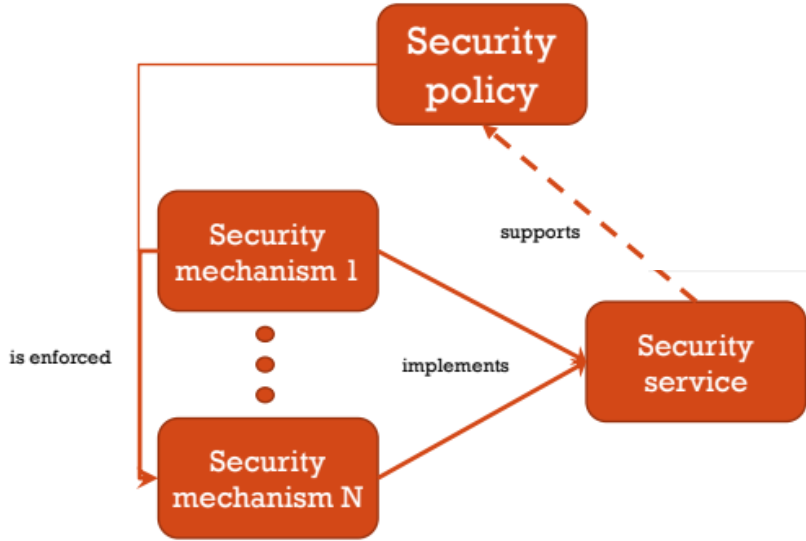
\includegraphics[height=10em]{01/schemaSecurity.png}
\section{CIA, Security Violation, and Mitigation}
    \paragraph{} La triade CIA non è solo essenziale per rendere sicuri i dati ma aiuta anche a capire cosa è andato storto nel caso di una \textbf{security violation}
    \subsection{Attacco Ransomware}
        \paragraph{L'arttacco}
            Nel caso di un attacco ransomware i dati vengono tenuti in ostaggio e la vittima viene ricattata con la pubblicazione di dati personali o il mancato accesso ad essi fino a che un riscatto non viene pagato.

            Questo attacco cripta i dati rendendoli inaccessibili e per ripristinarli è necessaria una chiave di decodifica, i pagamenti solitamente vengono eseguiti in crypto valute poco tracciabili.

            Questo genere di attacco viola la \textbf{confidentiality} e la \textbf{availability} dei dati.
        \paragraph{Mitigation}
            Per mitigare il rischio (che comunque non può essere eliminato) è utile procedere con un approccio \textbf{Zero Thrust} ovvero un "protocollo" che richiede che tutti gli utenti all'interno e all'esterno della rete aziendale siano autenticati e che la connessione è continuamente validata, prima di consentire accesso a applicazioni e dati.

\section{Risk}
    \paragraph{} Non esiste un sistema sicuro, esistono solo diversi livelli di insicurezza, si punta sempre ad ottenere il miglior livello di sicurezza possibile con il budget a disposizione.
    \subsection{Vulnerability}
        \subsubsection{Definizione}
            Una \textbf{vulnerabilità} è una debolezza in un sistema informativo, un sistema di sicurezza, nei controlli interni o nell'implementazione di questi. Questa debolezza può essere sfruttata o compromessa da una minaccia alla sicurezza.
        \subsubsection{Examples}
            Un esempio di \textbf{vulnerabilità} è una backdoor nascosta nel software e/o hardware, oppure dei bug non conosciuti di un software, o anche delle password deboli.
    \subsection{Threat}
        \subsubsection{Definizione}
            Qualunque circostanza o evento con il potenziale per causare perdite o danni a: operazioni dell'azienda, risorse o individui che possono accedere a tali risorse tramite un accesso non autorizzato, distruzione, pubblicazione, modifica e/o DoS. Inoltre un \textbf{threat} è un potenziale attacco che sfrutta una \textbf{vulnerabilità} del sistema.
        \subsubsection{Examples}
                Un esempio di \textbf{threat} sono:
                \begin{itemize}
                    \item Hacker:
                        \begin{itemize}
                            \item Trova e/o \textbf{sniff} una password.
                            \item Una il \textbf{social engineering} per ottenere informazioni sensibili e password.
                            \item Occupa le risorse di sistema con richieste inutili (attacchi DoS).
                        \end{itemize}
                    \item Virus e worms:
                        \begin{itemize}
                            \item I \textbf{virus} sono programmi auto replicanti che richiedono una azione dell'utente per essere attivati, esempio ne è una Email, un allegato o un link o un Floppy/CD/USB infetto.
                            \item I \textbf{worms} sono programmi auto replicanti che non richiedono una azione dell'utente per essere attivati, esempio ne è un worm che sfrutta una vulnerabilità di un sistema operativo.
                        \end{itemize} 
                \end{itemize}
    \subsection{Attack}
        \subsubsection{Definizione} Un \textbf{attacco} è un qualsiasi attività dannosa che prova a raccogliere, degradare, negare o distruggere informazioni o servizi. Può anche manifestarsi sotto un tentativo di ottenere un accesso ad una risorsa alla quale non si ha diritto 
    \subsection{Risk}
        \subsubsection{Definizione}
            Il \textbf{rischio} è la \textbf{probabilità} che una particolare \textbf{minaccia} \textbf{sfrutti} una particolare \textbf{vulnerabilità}.Il \textbf{rischio} è inoltre una misura di quanto una particolare circostanza o evento possa essere potenzialmente minacciato ed è tipicamente in funzione di: 
            \begin{enumerate}
                \item L'impatto che questa circostanza o evento potrebbe avere
                \item La probabilità che questa circostanza o evento si verifichi
            \end{enumerate}
        \subsubsection{Riassumendo}
            Riassumendo le \textbf{minacce} sono una combinazione di \textbf{intento} e \textbf{capability} di un attacco con successo. Invece le \textbf{vulnerabilità} sono caratterizzate da quanto è facile \textbf{identificarle} e \textbf{sfruttarle}.
            
            C'è da dire che l'impatto di un attacco deve essere valutato dal punto di vista di ogni soggetto coinvolto, ad esempio un attacco che compromette la privacy di un singolo individuo può avere un impatto molto diverso se lo si guarda dal punto di vista dell'individuo o dell'azienda.
        \subsubsection{Risk Matrix}
            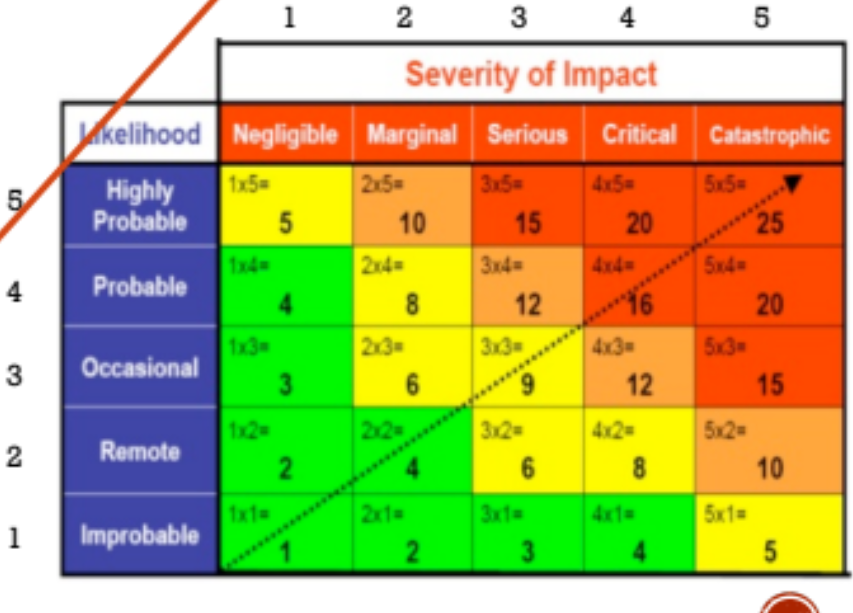
\includegraphics[height=10em]{01/riskMatrix.png}
            
            La presente matrice è una rappresentazione grafica del rischio, in cui si valuta la probabilità di un attacco e l'impatto che questo avrebbe, solitamente un rischio per essere accettabile deve avere un valore risultante tra basso (1-4) e medio-basso (5-9), i valori quali medio-alto (10-14) e alto (15-25) sono considerati inaccettabili e quindi devono essere mitigati abbassando la probabilità di attacco e/o l'impatto che questo avrebbe.

\section{Fine della diffusione degli attacchi}
    \paragraph{Generalmente} Il rischio è causato dunque dalla somma di una minaccia e una vulnerabilità, la minaccia è la capacità di sfruttare una vulnerabilità per causare un danno. 
    \paragraph{Pianizifazione} Quando si studiano i rischi sia prima che dopo un attacco bisogna considerare che se la \textbf{Minaccia - Threat} riesce a sfruttare la \textbf{Vulnerabilità - Vulnerability} allora si ha un \textbf{Rischio - Risk} se questo risulta inaccettabile allora si deve procedere con la \textbf{Mitigazione - Mitigation} del rischio, ciò riduce la \textbf{Minaccia - Threat} e il ciclo riprende fino a quando il \textbf{Rischio residuo - Residual Risk} è accettabile.

\section{Security \& Human Factor - Sicurezza \& Fattore Umano}
    Il fattore umano è uno dei fattori più importanti nella sicurezza informatica, infatti la maggior parte degli attacchi sono causati da password poco sicure o da una mancata preparazione degli utenti.
    \subsection{Passwords}
        C'è chi dice che le password andrebbero trattate come la biancheria intima, ovvero:
        \begin{itemize}
            \item Cambiate regolarmente - magari senza usare un pattern
            \item Non condivise con nessuno - nemmeno con colleghi o familiari
            \item Non lasciate sulla scrivania - non scritte su post-it o in chiaro
        \end{itemize}
    \subsection{Security}
        Ogni persona che ha accesso ad un sistema informatico è un potenziale punto di attacco, quindi è importante che ogni utente sia formato sulla sicurezza, ogni utente al suo livello a partire dall'utente base che necessita di una formazione base fino ad arrivare all amministratore di sistema che necessita di una formazione più avanzata.
    \chapter{Authentication I: Passwords \& co}
\thispagestyle{chapterInit}
\section{User Authentication \& Digital Identity - Autenticazione e Identità Digitale}
    \label{sec:user-authentication}
    \subsection{Introduzione e Definizioni}
        \begin{description}
            \item[Identità] è un insieme di attributi relazionati ad una entità
            \item[Attributo] è una caratteristica o proprietà di una entità ch e può essere usata per descriverne lo stato, apparenza o ogni altro aspetto.  
            \item[Identità digitale] è ua identità i quali attributi sono conservati e trasmessi in forma digitale 
        \end{description}
        Ma perché la identità digitale è importante? In pratica questa può essere una soluzione per diversi aspetti che i governi mondiali vorrebbero risolvere.
    \subsection{Digital Identity Lifecycle - Ciclo di Vita dell'Identità Digitale}
        \begin{description}
            \item[Creazione] L'identità viene creata, in genere da un ente di certificazione che assicura l'identità dell'utente e fornisce/chiede una forma di accesso per riconoscere in futuro l'utente. Viene creato un ID univoco per l'utente
            \item[Autenticazione] L'identità viene autenticata tramite il metodo concordato in fase di creazione
            \item[Autorizzazione/ Accesso] L'utente ha accesso a risorse e servizi in base ai permessi assegnati, i dati necessari dell'utente vengono trasmessi dall'ente di certificazione al servizio.
            \item[Cancellazione o Disattivazione] L'identità viene cancellata o disattivata quando non è più necessaria e i dati devono essere cancellati dopo un certo periodo di tempo per garantire la privacy dell'utente.
        \end{description}
        \subsubsection{Enrollment / On-Boarding - Creazione}
            La fase di creazione di una utenza porta un \textbf{Applicant} a diventare un \textbf{Subscriber} tramite una serie di passaggi:
            \begin{description}
                \item[Resolution] Vengono raccolti gli \textbf{attributi} essenziali dell'utente (nome, indirizzo, data e luogo di nascita, \dots) vengono ora raccolti anche due documenti di identità (patente, passaporto, C.I.,\dots) - ora l'utente viene distinto univocamente su un contesto
                \item[Validation] Gli \textbf{attributi} raccolti vengono validati sulla base di \textbf{prove} tramite una fonte autorevole- gli attributi vengono ora associati ad una persona fisica 
                \item[Verification] Le \textbf{prove} vengono verificate, in questo punto si verifica la corrispondenza tra le diverse foto, viene mandato un codice ai contatti per verificare che siano i suoi, etc - l'utente viene ora confermato e la sua identità è certificata 
            \end{description}
            \paragraph{Identity Assurance Levels - Livelli di Assicurazione dell'Identità}
                \begin{description}
                    \item[IAL1] GLi attributi, se presenti, vengono auto-dichiarati, o considerati come tali
                    \item[IAL2] Una persona o di remoto o in presenza, verifica gli attributi
                    \item[IAL3] Gli attributi vengono verificati da una persona autorizzata e i documenti fisici vengono esaminati
                \end{description}  
        \subsubsection{Authentication - Autenticazione}
            \paragraph{Definzione} L'\textbf{autenticazione} è il processo di verifica dell'identità di un utente, processo o dispositivo.

            Il \textbf{richiedente} deve dimostrare al \textbf{verificante} che è chi dice di essere.
            \paragraph{Base} Quando esegui il login solitamente inserisci un \textbf{username} e una \textbf{password} che vengono confrontati con quelli memorizzati nel sistema.

            L'autenticazione tramite \textbf{password} è molto diffusa e semplice da implementare.
\section{An Introduction to Passwords - Introduzione alle Password}
    \subsection{User Authn - Autenticazione Utente}
        Quando esegui il login inserisci un \textbf{username} per annunciare chi sei e una \textbf{password} per dimostrare chi dici di essere, questo tipo di autenticazione si chiama \textbf{user authn} ovvero il processo di verifica dell'identità di un utente.
        \subsubsection{Entollment - Creazione}
            Le \textbf{password} dovrebbero essere conosciute solo dall'utente e dal sistema. Spesso però, soprattutto nelle grandi aziende, le password vengono mandata via mail o scritte dall'utente su una pagina web. In questi casi da chi potrebbe essere intercettata la password?
        \subsubsection{La teoria rispetto alla realtà}
            Le password hanno dominato il mondo dell'informatica sin dall'avvento dei computer, ma da allora la richiesta verso queste è che siano più sicure ma allo stesso tempo più "User Friendly", siamo in ricerca di alternative ma per ora delle proposte alternative come \textit{criteri di complessità} ma studi hanno rilevato che spesso non vengono rispettati e/o che non sono efficaci. 
    \subsection{Password Security - Sicurezza delle Password}
        All'inizio di internet le password venivano conservate in file appositi in chiaro, ma questo comportava un rischio molto alto, infatti se un attaccante riusciva ad accedere a quel file poteva facilmente accedere a tutte le password.

        \subsubsection{Hashing}
            Per risolvere questo problema si è pensato di "\textbf{hash-are}" le password, ovvero di applicare una funzione di hash alla password e conservare il risultato. In questo modo se un attaccante accede al file delle password non può risalire alla password originale.
            \paragraph{Proprietà della funzione di hash}
                Una funzione di hash ottimale dovrebbe avere le seguenti proprietà:
                \begin{description}
                    \item[Deterministica] dato un input la funzione restituisce sempre lo stesso output
                    \item[Rapida] la funzione deve essere veloce da calcolare
                    \item[Difficile da invertire] data l'output è difficile risalire all'input
                    \item[Biettiva] due input diversi devono avere output diversi
                    \item[Lunghezza fissa] l'output deve avere una lunghezza fissa indipendentemente dalla lunghezza dell'input
                \end{description}
                Molto spesso però capita che i bit disponibili per l'hash siano limitati rispetto a tutti i possibili input, per questo motivo si è cercato di creare funzioni di hash che generano due output uguali solo in rarissimi casi, inoltre si aggiunge a questo che per input simili l'output sia molto diverso.
            \subsubsection{Crack of Passwords}
                In caso di un "leak" di password che sono state opportunamente codificate con una funzione di hash, un attaccante può tentare di decifrarle ma questo è molto difficile. Questo diventa più semplice se vengono usate password poco sicure e/o comuni. infatti si stimi che per  trovare una password da 8 caratteri composti da lettere minuscole e numeri ci vogliano "solo" 155€ su una istanza di AWS.
        \subsection{Hash \& Salt}
            Per rendere più difficile il lavoro degli attaccanti si è pensato di aggiungere un \textbf{salt} alle password, ovvero un valore casuale che viene aggiunto alla password prima di calcolare l'hash. Questo rende più difficile per l'attaccante decifrare la password.
\section{Multi Factor Authentication - Autenticazione a più fattori}
\label{sec:mfa}
    \subsection{Definizione}
        L'autenticazione a più fattori è un metodo di autenticazione che richiede l'uso di più metodi di autenticazione per verificare l'identità di un utente.
    \subsection{Fattori di Autenticazione}
        I fattori di autenticazione sono:
        \begin{description}
            \item[Qualcosa che sai] (password, PIN, \dots)
            \item[Qualcosa che hai] (smartphone, token, \dots)
            \item[Qualcosa che sei] (impronte digitali, riconoscimento facciale, \dots)
        \end{description}
        \subsubsection{Vantaggi/Svantaggi quello che sai}
            \paragraph{Vantaggi}
                \begin{itemize}
                    \item Facile da implementare - non richiede hardware aggiuntivo
                    \item Facile da usare - Basta ricordare la password
                    \item Facile da resettare se dimenticato - basta fare il reset della password
                \end{itemize}
            \paragraph{Svantaggi}
                \begin{itemize}
                    \item Facile da rubare - se un attaccante riesce a scoprire la password può accedere al sistema 
                    \item Facile da dimenticare - se la password è complessa è facile dimenticarla
                    \item Facile da indovinare - se la password è semplice ed è stata usata in altri contesti è facile indovinarla
                \end{itemize}
        \subsubsection{Vantaggi/Svantaggi quello che hai}
            \paragraph{Vantaggi}
                \begin{itemize}
                    \item Difficile da rubare - se un attaccante non ha il dispositivo non può accedere al sistema
                    \item Difficile da indovinare - se il dispositivo è protetto da PIN o password è difficile indovinare l'accesso
                    \item Difficile da clonare - se il dispositivo è protetto da un token è difficile clonarlo inoltre la parte di autenticazione è fatta dal dispositivo stesso e non dal sistema
                \end{itemize}
            \paragraph{Svantaggi}
                \begin{itemize}
                    \item Facile da perdere - se il dispositivo viene perso l'utente non può accedere al sistema
                    \item Difficile da resettare - se il dispositivo viene perso l'utente deve contattare l'amministratore per resettare l'accesso
                    \item Costoso - i dispositivi possono essere costosi 
                \end{itemize}
        \subsubsection{Vantaggi/Svantaggi quello che sei}
            \paragraph{Vantaggi}
                \begin{itemize}
                    \item Difficile da rubare - le impronte digitali o il riconoscimento facciale sono unici e difficili da rubare
                    \item Difficile da indovinare - è difficile indovinare le impronte digitali o il riconoscimento facciale
                    \item Difficile da clonare - è difficile clonare le impronte digitali o il riconoscimento facciale
                \end{itemize}
            \paragraph{Svantaggi}
                \begin{itemize}
                    \item Se il fattore viene compromesso non può essere cambiato - se le impronte digitali vengono rubate non possono essere cambiate
                    \item Costoso - i dispositivi possono essere costosi
                    \item Non sempre preciso - il riconoscimento facciale può essere ingannato
                \end{itemize}
        \subsubsection{PSD2 Compliance}
            \paragraph{Cos'è PSD2} La \textbf{PSD2} è una direttiva europea che regola i servizi di pagamento e che richiede l'autenticazione a più fattori per i pagamenti online. Questo per ridurre il rischio di frodi.
            \paragraph{How to comply MFA in PSD2} Una idea sarebbe quella di includere nella challenge anche i dati della particolare transazione come:
                \begin{itemize}
                    \item L'identificativo del destinatario della transazione
                    \item L'importo della transazione
                    \item L'instante nella quale la transazione è stata inizializzata
                    \item \dots
                \end{itemize}
            Purtroppo però ciò non è abbastanza in quanto i dati sopra indicati possono essere ricavati dal contesto il che rende la challenge prevedibile.
    \subsection{FIDO: Phishing Resistant Authentication}
        \subsubsection{Cos'è FIDO}
            \textbf{FIDO (Fast Identity Online)} è un insieme di standard aperti per l'autenticazione a più fattori che mira a ridurre il rischio di phishing. Il suo scopo è quello di assicurare una \textbf{autenticazione forte} e di \textbf{ridurre l'uso di password}.
        \subsubsection{Come funziona}
            \begin{enumerate}
                \item Viene chiesto all'utente di scegliere un ente FIDO
                \item L'utenti sblocca il dispositivo FIDO usando un'impronta digitale, un pulsante su un dispositivo di secondo fattore, un PIN o un qualsiasi altro metodo di autenticazione supportato
                \item Il dispositivo crea una chiave pubblica e una chiave privata univoca per il dispositivo, il servizio online e l'utente
                \item La chiave pubblica è inviata al servizio online ed associata all'account dell'utente
                \item Il servizio online chiede all'utente di autenticarsi con il dispositivo precedentemente registrato
                \item L'utente sblocca il dispositivo FIDO usando lo stesso metodo di autenticazione usato in precedenza
                \item Il dispositivo FIDO usa l'account dell'utente identificato per inviare la corretta chiave al servizio online
                \item Infine il dispositivo invia la challenge ricevuta dal servizio online firmata con la chiave privata e il servizio online verifica la firma con la chiave pubblica, l'utente è autenticato.
            \end{enumerate}
\section{Outsourcing Authentication}
    \label{sec:outsourcing-authentication}
    \subsection{Definizione}
        L'outsourcing dell'autenticazione è il processo di affidare l'autenticazione degli utenti ad un servizio esterno, spesso chiamato \textbf{Identity Provider}. Questo servizio si occupa di verificare l'identità dell'utente e di inviare un token di autenticazione al servizio che richiede l'autenticazione. Esempio in italia per l'accesso ai servizi pubblici si usa SPID.
    \subsection{Che problema risolve}
        L'outsourcing dell'autenticazione risolve diversi problemi:
        \begin{description}
            \item[Sicurezza] L'Identity Provider è specializzato in autenticazione e può offrire un livello di sicurezza più alto
            \item[User Experience] L'Identity Provider può offrire un'esperienza utente migliore in quanto l'utente non deve ricordare le password per ogni servizio ma solo quella dell'Identity Provider - SSO
            \item[Compliance] L'Identity Provider può aiutare a rispettare le normative sulla privacy e la sicurezza
        \end{description}
    \subsection{La soluzione}
        L'outsourcing dell'autenticazione è delegato ad una terza parte, l'\textbf{Identity Provider}, che si occupa di verificare l'identità dell'utente e di inviare le informazioni di autenticazione al servizio che richiede l'autenticazione. A questo punto il servizio invia all'utente un token di autenticazione che può essere usato per accedere al servizio senza dover inserire nuovamente le credenziali del SSO.
    \subsection{Potenziali Problemi}
        L'outsourcing dell'autenticazione può comportare alcuni problemi:
        \begin{description}
            \item[Single Point of Failure] Se l'Identity Provider è compromesso tutti i servizi che usano l'Identity Provider per l'autenticazione sono compromessi
            \item[Privacy] L'Identity Provider può raccogliere informazioni sull'utente e sulle sue abitudini di navigazione
        \end{description}
    \chapter{Cryptography Introduction}
\section{Cryptosystem}
    \paragraph{Definizione} Un \textbf{cryptosystem} è una tupla di 5 elementi (E,D,M,K,C):
    \begin{description}
        \item[E] è un \textit{algoritmo di cifratura}
        \item[D] è un \textit{algoritmo di de-cifratura}
        \item[M] è un insieme di \textit{messaggi in chiaro}
        \item[K] è un insieme di \textit{chiavi}
        \item[C] è un insieme di \textit{messaggi cifrati}
    \end{description}
    In modo astratto i punti \textbf{E} e \textbf{D} possono essere espresse come funzioni:
    $$
        \begin{aligned}
            E: M \times K \rightarrow C \\
            D: C \times K \rightarrow M
        \end{aligned}
        \qquad D(E(m,k),k) = m
    $$
    Nella criptografia base ogni chiave $ k \in K $ può essere usata per cifrare e de-cifrare i messaggi, nella criptografia simmetrica la chiave è la stessa per entrambi i processi, mentre nella criptografia asimmetrica le chiavi sono diverse.
    \paragraph{Quali componenti sono pubbliche?} Solitamente non abbiamo necessità di mantenere segrete le funzioni \texttt{E} e \texttt{D} o il messaggio cifrato \texttt{C}, quello che davvero deve essere segreto è la chiave \texttt{K}. Il motivo per il quale le funzioni non devono essere segrete è che il sistema deve essere pubblico e quindi tramite processi di \textit{reverse engineering} è possibile ricavare le funzioni (es: il sistema di cifratura di un DVD è stato ricavato tramite \textit{reverse engineering} dopo solo due giorni).
    \subsection{Why Cryptography?}
        \paragraph{Sicurezza} La crittografia è usata nei \hyperref[subsec:securityMechanism]{\textbf{meccanismi di sicurezza}} per garantire \hyperref[subPar:confidentiality]{\textbf{confidenzialità}} nascondendo il contenuto dei messaggi, \hyperref[subPar:integrity]{\textbf{integrità}} provvedendo al controllo di integrità tramite funzioni di \textbf{hash} e \textbf{la verifica dell'origine} dei dati tramite firme digitali verificabili da una fonte autorevole.
    \subsection{Cryptography on rented servers}
        \paragraph{Problema} Se si usa un server di terze parti per conservare dati, ad esempio su un database, è possibile che il proprietario del server possa accedere ai dati in chiaro. Per evitare ciò si può cifrare i dati prima di inviarli al server, in modo che il proprietario non possa leggerli, ciò comporta però un aumento del carico computazionale lato client in quanto tutti i dati prima di essere letti devono essere de-cifrati, per questo esistono meccanismi di ricerca su dati cifrati che permettono di effettuare ricerche su dati cifrati senza de-cifrarli, una volta trovati i dati desiderati si de-cifrano solo quelli.
    \subsection{Come definiamo "Computazionalmente sicuro" nelle comunicazioni}
        \paragraph{Definzizione} Definiamo un sistema di comunicazione \textbf{Computazionalmente sicuro} quando la decifrazione di un messaggio cifrato senza conoscere la chiave è molto difficile, o addirittura impossibile, e richiede molto tempo e risorse computazionali.
        \paragraph{$E(k,P)=C$} Calcolare $C$ da $P$ deve essere difficile senza $k$, inoltre calcolare $C$ da $P$ sapendo $k$ deve essere facile.
        \paragraph{$D(k,C)=P$} Calcolare $P$ da $C$ deve essere facile sapendo $k$, ma deve essere difficile senza $k$.
        \paragraph{Trapdoor - funzione a senso unico} Una \textbf{trapdoor} è una funzione a senso unico che richiede una ulteriore informazione. Ed una \textbf{funzione a senso unico} è descritta come una funzione che è facile da calcolare in una direzione, ma molto più difficile nell'altra.  
    \subsection{Hash v/s Encryption}
        \paragraph{Quando l'una e quando l'altra} Usiamo funzioni di hash quando non abbiamo bisogno di accedere all'informazione originale, ma solo di verificare l'integrità dei dati. Ricordiamo che le funzioni di \textbf{hash} per definizione sono \textbf{one-way} e \textbf{deterministiche}, quindi non possiamo de-cifrarle e non necessitiamo di una chiave per cifrare i dati. \newline
        D'altro canto usiamo la cifratura quando i dati che vogliamo proteggere devono poter essere letti e ne vogliamo preservare la \textbf{confidenzialità}, bisogna prima concordare una \textbf{chiave} in maniera sicura, poi calcolare il \textbf{messaggio cifrato} con suddetta chiave e infine inviare il messaggio cifrato, il destinatario potrà de-cifrare il messaggio con la chiave concordata. In questo modo proteggiamo la \textbf{confidenzialità} e la \textbf{riservatezza} dei dati ma non la loro \textbf{integrità}.
    \subsection{La Criptografia non è la soluzione a tutti i problemi}
        \paragraph{Perchè?} La crittografia non è la soluzione a tutti i problemi di sicurezza, in quanto comunque è sensibile a delle chiavi conservate su supporti digitali, i quali devono proteggere questa informazione. Inoltre da sola la crittografia non è mai usata come soluzione a problemi di sicurezza, ma sempre in combinazione con altri meccanismi di sicurezza.
\section{Types of cryptography - Tipologie di criptografia}
    \subsection{Cifrari di sostituzione}
        \paragraph{In breve} I \textbf{cifrari di sostituzione} sono cifrari che sostituiscono un simbolo del \textit{dizionario} con un altro simbolo. In questo contesto la \textit{chiave} è la \textit{sostituzione} dei simboli.
        \paragraph{In lungo}
            I \textbf{cifrari di sostituzione} sono dei \textbf{metodi di criptazione} per i quali ogni simbolo del \textbf{messaggio in chiaro} è rimpiazzato nel \textbf{messaggio cifrato} rispetto ad un prefissato sistema. I "simboli" possono essere lettere, coppie di lettere, triple di lettere, o anche una combinazione di questi, e anche altro. Il ricevente decifra il testo svolgendo le sostituzioni inverse.
        \subsubsection{Cifrario di cesare}
            Il \textbf{cifrario di Cesare} è un cifrario di sostituzione in cui il \textbf{dizionario} del testo in chiaro è spostato di un numero fisso di posizioni nell'alfabeto. Per decifrare il testo cifrato si sposta indietro dello stesso numero di posizioni.\newline
            Questo tipo di sistema viene anche chiamato: \textbf{rotazione di $k$ posizioni}, in quanto il dizionario viene ruotato di $k$ posizioni.
            \paragraph{Problemi e proprietà} Il cifrario descritto è il più semplice tra tutti come decodifica in quanto esistono solo $25$ chiavi e con un semplice attacco di \textbf{brute force}. Inoltre se non si vuole usare un attacco di \textbf{brute force} si può comunque cercare di trovare lettere comuni del messaggio cifrato e provare a ricondurle a lettere comuni dell'alfabeto.
            \begin{figure}[H]
                \centering
                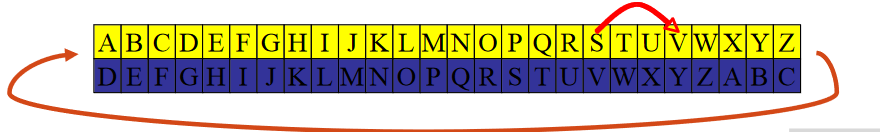
\includegraphics[width=0.9\textwidth]{03/cifrarioCesare.png}
                \caption{Esempio di cifrario di Cesare spostato di 3 posizioni}
            \end{figure}
        \subsubsection{Cifrario di Vigenère}
            Il \textbf{cifrario di Vigenère} è un cifrario che prevede l'uso di una "parola chiave", se necessario ripetuta per la lunghezza del messaggio, per poi calcolare la "somma" dei valori di ogni lettera del messaggio con la corrispondente lettera della parola chiave (prendendo poi il resto della divisione per 26). Quindi assegnando ad ogni lettera un numero da 0 a 25, si somma il numero della lettera del messaggio con il numero della lettera della parola chiave, si prende il resto della divisione per 26 e si assegna alla lettera corrispondente il numero ottenuto.
            \begin{figure}[H]
                \centering
                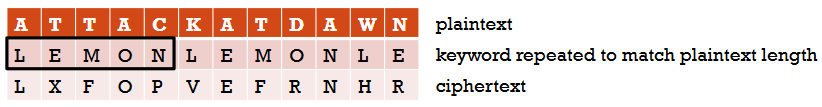
\includegraphics[width=0.9\textwidth]{03/cifrario2.png}
                \caption{Esempio di cifrario di Vigenère chiave "lemon"}
            \end{figure}
            Per decifrare il messaggio cifrato si sottrae il numero della lettera della parola chiave al numero della lettera del messaggio e si prende il resto della divisione per 26.
            \paragraph{Vantaggi} Questo cifrario è molto più sicuro rispetto a quello di cesare in quanto come mostrato nell'esempio la lettera "A" viene codificata in quattro lettere diverse e la lettera "T" che è presente tre volte viene cifrata in due lettere corrispondenti. In quanto la parola chiave ha lunghezza "l" allora dimensione della chiave è $l^{26}$. Inoltre se la chiave è della stessa lunghezza del messaggio allora il cifrario di Vigenère è equivalente a un cifrario di sostituzione casuale il che rende impossibile la decifrazione, però ciò comporta ad una ulteriore difficoltà per il mittente e il destinatario nel concordare una chiave.
    \subsection{Cifrari di trasposizione}
        \paragraph{In breve} I \textbf{cifrari di trasposizione} sono cifrari che permutano i simboli del messaggio in chiaro. In questo contesto la \textit{chiave} è la \textit{permutazione} dei simboli.
        \paragraph{In lungo} I \textbf{cifrari di trasposizione} sono dei \textbf{metodi di criptazione} per i quali i simboli del \textbf{messaggio in chiaro} sono permutati in un certo modo per ottenere il \textbf{messaggio cifrato}. Il ricevente decifra il testo svolgendo le permutazioni inverse.
        \subsubsection{Cifrario di trasposizione per colonne}
            Il \textbf{cifrario di trasposizione per colonne} è un cifrario che permuta i simboli del messaggio in chiaro per colonne, in modo che il messaggio cifrato sia una matrice di colonne.
            \begin{figure}[H]
                \centering
                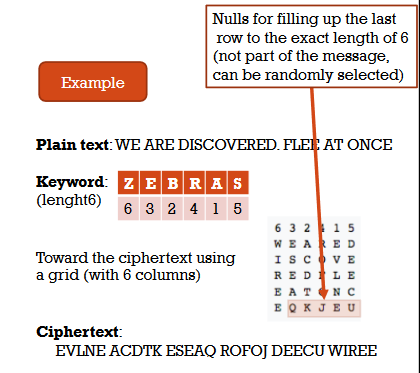
\includegraphics[width=0.5\textwidth]{03/cifrario3.png}
                \caption{Esempio di cifrario di trasposizione per colonne}
            \end{figure}
            Per decifrare il messaggio cifrato si riordinano le colonne in base alla chiave.
    \subsection{Criptografia Simmetrica}
        Come detto in precedenza la \textbf{criptografia simmetrica} prevede la stessa \textbf{chiave} per cifrare e de-cifrare i messaggi. La gestione di chi possiede le chiavi determina chi può accedere ai dati.
        \paragraph{Tipi} Esistono nella \textit{criptografia moderna} due tipi ci crittografia simmetrica:
        \begin{description}
            \item[Cifrari a flusso] I \textbf{cifrari a flusso} cifrano una "breve" porzione di un blocco di dati alla volta con una chiave che varia nel tempo. Questa tipologia si base su un \textbf{generatore di chiavi}, la cifratura è relativamente semplice (es. \texttt{XOR}) e molto spesso viene usato un bit per blocco.
            \item[Cifrari a blocchi] I \textbf{cifrari a blocchi} cifrano un blocco di dati "lungo" alla volta con una chiave fissa. Questa tipologia è più complessa e richiede uan funzione di cifratura e una di de-cifratura. Solitamente si usano blocchi di 64/128 bit.  
        \end{description}
        \subsubsection{Cifrari a flusso}
            I cifrari a flusso operano su un flusso di testo in chiaro e producono un flusso di testo cifrato. Lo stesso testo se ripetuto può essere cifrato in modo diverso in base al tempo nel quale è stato cifrato. I circuiti sono molto semplici e progettati per essere molto veloci.
            \begin{figure}[H]
                \centering
                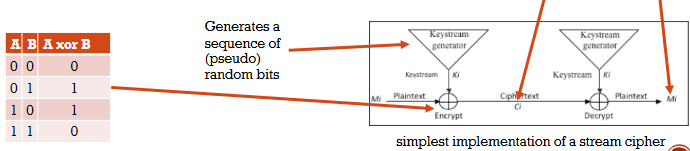
\includegraphics[width=0.9\textwidth]{03/cifrarioFlusso.png}
                \caption{Esempio di circuito di cifratura a flusso}
            \end{figure}
            \paragraph{Dove si usano} I cifrari a flusso sono usati in applicazioni in cui la velocità è fondamentale, come ad esempio nelle comunicazioni via radio o nella comunicazione in tempo reale.
        \subsubsection{Cifrari a blocchi}
\end{document}